% Copyright (C) 2012 Shi.Zhan <g.shizhan.g@gmail.com>
%
% Permission is hereby granted, free of charge, to any person obtaining a copy of this software and associated documentation files (the "Software"), to deal in the Software without restriction, including without limitation the rights to use, copy, modify, merge, publish, distribute, sublicense, and/or sell copies of the Software, and to permit persons to whom the Software is furnished to do so, subject to the following conditions:
%
% The above copyright notice and this permission notice shall be included in all copies or substantial portions of the Software.
%
% THE SOFTWARE IS PROVIDED "AS IS", WITHOUT WARRANTY OF ANY KIND, EXPRESS OR IMPLIED, INCLUDING BUT NOT LIMITED TO THE WARRANTIES OF MERCHANTABILITY, FITNESS FOR A PARTICULAR PURPOSE AND NONINFRINGEMENT. IN NO EVENT SHALL THE AUTHORS OR COPYRIGHT HOLDERS BE LIABLE FOR ANY CLAIM, DAMAGES OR OTHER LIABILITY, WHETHER IN AN ACTION OF CONTRACT, TORT OR OTHERWISE, ARISING FROM, OUT OF OR IN CONNECTION WITH THE SOFTWARE OR THE USE OR OTHER DEALINGS IN THE SOFTWARE.
%
% 课程:人机交互技术及应用
% 班级:传播学1001班
% 课时:40学时,2012年秋季1~10周,每周一、三
% 地点:东九楼D212
% 主页:http://code.google.com/p/hci-course/
% 教师:施展 
% 单位:华中科技大学 武汉光电国家实验室
%
\documentclass{beamer}
\usepackage{fontspec,xunicode,xltxtra,beamerthemesplit}
%\usetheme{Hannover} % White background
\usetheme{Berkeley} % Blue background
\setmainfont[
	BoldFont={WenQuanYi Zen Hei},
	ItalicFont={WenQuanYi Micro Hei}
]{WenQuanYi Micro Hei}
\setsansfont[
	BoldFont={WenQuanYi Zen Hei},
	ItalicFont={WenQuanYi Micro Hei}
]{WenQuanYi Micro Hei}

% 中文环境自动换行
\XeTeXlinebreaklocale "zh"
\XeTeXlinebreakskip = 0pt plus 1pt

% 中文环境修正导航栏
\makeatletter
\def\beamer@linkspace#1{
	\begin{pgfpicture}{0pt}{-1.5pt}{#1}{5.5pt}
		\pgfsetfillopacity{0}
		\pgftext[x=0pt,y=-1.5pt]{.}
		\pgftext[x=#1,y=5.5pt]{.}
	\end{pgfpicture}
}
\makeatother

% diagrams
\usepackage{tikz}
\usetikzlibrary{arrows,shapes}

% full page image
\newcommand{\fullPageImage}[2]{
	{
		\usebackgroundtemplate{\includegraphics[width=\paperwidth, height=\paperheight]{#1}}
		\frame[plain]{#2}
	}
}

\title{人机交互技术}
\author{施展}
\institute{华中科技大学~武汉光电国家实验室}
\date{\today}
\titlegraphic{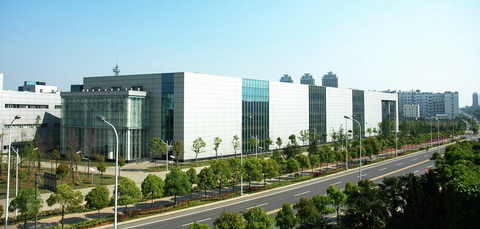
\includegraphics[width=2cm]{images/wnlo.jpg}}

\begin{document}

\begin{frame}
	\titlepage
\end{frame}

\begin{frame}
	\frametitle{内容提要}
	\tableofcontents
\end{frame}

\section{第七讲}
\begin{frame}
	\frametitle{第七讲 Web界面设计}
	\begin{itemize}
		\item 熟悉Web设计的原则及Web界面设计包含的元素。
		\item 掌握Web界面设计语言和技术,并灵活应用。
		% adjust to html5, introduce the most recent and promising techonology
	\end{itemize}
\end{frame}

\subsection{Web界面及相关概念}
\begin{frame}
	\frametitle{Web界面及相关概念}
	\beamertemplatetransparentcovereddynamicmedium
	\begin{itemize}[<+->]
		\item 万维网 World Wide Web, WWW
		\begin{itemize}
			\item 由高能核物理学家Tim Berners-Lee建立雏形:
			\begin{itemize}
				\item 一个能够整合各种资源、文件及多媒体的系统,让使用者方便地取得不同媒体的资料。
			\end{itemize}
			\item 建立在客户/服务器模型之上
			\begin{itemize}
				\item 超文本标记语言 Hypertext Markup Language, HTML~\cite{berners1995hypertext}
				\item 超文本传输协议 Hypertext Transport Protocols, HTTP~\cite{fielding1999hypertext}
				\item 通过Internet把遍布世界各地的服务器连接起来,提供各种服务,具有一致用户界面的信息浏览功能。
			\end{itemize}
		\end{itemize}
	\end{itemize}
\end{frame}

\begin{frame}
	\frametitle{Web的发展趋势}
	\beamertemplatetransparentcovereddynamicmedium
	\begin{itemize}
		\item Web的爆炸性发展
		\begin{itemize}
			\item 各种媒体
			\item 各类交互
			\item 广泛渗透 
		\end{itemize}
		\pause
		\item W3C标准: XML
		\pause
		\item Web 2.0 \& 云
		\pause
		\item Web 3.0 \& Semantic Web
	\end{itemize}
\end{frame}

\begin{frame}
	\frametitle{超文本与超媒体}
	\beamertemplatetransparentcovereddynamicmedium
	\begin{itemize}
		\item 超文本 Hypertext
		\begin{itemize}
			\item 是一种使用于文本、图形或其他信息的组织形式,非线性的信息组织。
			\item 使得单一的信息元素之间可以相互交叉引用,这种引用并不是通过复制来实现的,而是通过指向对方的地址字符串来指引用户获取相应的信息。 
		\end{itemize}
		\pause
		\item 超媒体 Hypermedia
		\begin{itemize}
			\item 利用超文本形式组织起来的文件不仅仅是文本,也可以是图、文、声、像以及视频等多媒体形式的文件。
			\item 这些多媒体信息就构成了所谓的超媒体 。
		\end{itemize}
	\end{itemize}
\end{frame}

\begin{frame}
	\frametitle{Web界面设计问题的提出}
	\beamertemplatetransparentcovereddynamicmedium
	\begin{itemize}[<+->]
		\item Web界面设计与站点外观直接相关
		\begin{itemize}
			\item 站点的界面外观是否友好直接关系到是否能吸引人的关注。
		\end{itemize}
		\pause
		\item 人性化的设计是Web界面设计的核心
		\begin{itemize}
			\item 如何根据人的心理、生理特征,运用技术手段,创造简单、友好的界面,是Web界面设计的重点。
		\end{itemize}
	\end{itemize}
\end{frame}

\subsection{Web界面设计原则}
\begin{frame}
	\frametitle{Web界面设计原则}
	\beamertemplatetransparentcovereddynamicmedium
	\begin{enumerate}[<+->]
		\item 以用户为中心
		\item 一致性
		\item 简洁与明确
		\item 体现特色
		\item 兼顾不同的浏览器
		\item 明确的导航设计
	\end{enumerate}
\end{frame}

\begin{frame}
	\frametitle{Web界面设计原则~{\small 以用户为中心}}
	\beamertemplatetransparentcovereddynamicmedium
	\begin{itemize}[<+->]
		\item .
	\end{itemize}
\end{frame}

\begin{frame}
	\frametitle{Web界面设计原则~{\small 一致性}}
	\beamertemplatetransparentcovereddynamicmedium
	\begin{itemize}[<+->]
		\item .
	\end{itemize}
\end{frame}

\begin{frame}
	\frametitle{Web界面设计原则~{\small 简洁与明确}}
	\beamertemplatetransparentcovereddynamicmedium
	\begin{itemize}[<+->]
		\item .
	\end{itemize}
\end{frame}

\begin{frame}
	\frametitle{Web界面设计原则~{\small 体现特色}}
	\beamertemplatetransparentcovereddynamicmedium
	\begin{itemize}[<+->]
		\item .
	\end{itemize}
\end{frame}

\begin{frame}
	\frametitle{Web界面设计原则~{\small 兼顾不同的浏览器}}
	\beamertemplatetransparentcovereddynamicmedium
	\begin{itemize}[<+->]
		\item .
	\end{itemize}
\end{frame}

\begin{frame}
	\frametitle{Web界面设计原则~{\small 明确的导航设计}}
	\beamertemplatetransparentcovereddynamicmedium
	\begin{itemize}[<+->]
		\item .
	\end{itemize}
\end{frame}

\subsection{Web界面要素设计}
\begin{frame}
	\frametitle{Web界面要素设计}
	\beamertemplatetransparentcovereddynamicmedium
	\begin{enumerate}[<+->]
		\item Web界面规划
		\item 文化与语言
		\item 内容、风格与布局、色彩设计
		\item 文本设计
		\item 多媒体元素设计
	\end{enumerate}
\end{frame}

\begin{frame}
	\frametitle{Web界面要素设计~{\small Web界面规划}}
	\beamertemplatetransparentcovereddynamicmedium
	\begin{itemize}[<+->]
		\item .
	\end{itemize}
\end{frame}

\begin{frame}
	\frametitle{Web界面要素设计~{\small 文化与语言}}
	\beamertemplatetransparentcovereddynamicmedium
	\begin{itemize}[<+->]
		\item .
	\end{itemize}
\end{frame}

\begin{frame}
	\frametitle{Web界面要素设计~{\small 内容、风格与布局、色彩设计}}
	\beamertemplatetransparentcovereddynamicmedium
	\begin{itemize}[<+->]
		\item .
	\end{itemize}
\end{frame}

\begin{frame}
	\frametitle{Web界面要素设计~{\small 文本设计}}
	\beamertemplatetransparentcovereddynamicmedium
	\begin{itemize}[<+->]
		\item .
	\end{itemize}
\end{frame}

\begin{frame}
	\frametitle{Web界面要素设计~{\small 多媒体元素设计}}
	\beamertemplatetransparentcovereddynamicmedium
	\begin{itemize}[<+->]
		\item .
	\end{itemize}
\end{frame}

\subsection{Web界面基本技术}
\begin{frame}
	\frametitle{Web界面基本设计技术}
	\beamertemplatetransparentcovereddynamicmedium
	\begin{itemize}[<+->]
		\item 超文本标记语言 HTML
		\item 富英特网应用 Rich Internet Application 
		\item 客户端脚本语言 JavaScript 
		\item 服务器端脚本语言 Dynamic Web Page
		\item 服务器端 JavaScript
	\end{itemize}
\end{frame}

\begin{frame}
	\frametitle{Web界面基本技术~{\small HTML}}
	\beamertemplatetransparentcovereddynamicmedium
	\begin{itemize}[<+->]
		\item .
	\end{itemize}
\end{frame}

\begin{frame}
	\frametitle{Web界面基本技术~{\small RIA}}
	\beamertemplatetransparentcovereddynamicmedium
	\begin{itemize}[<+->]
		\item JavaApplet, Flash, Silverlight
	\end{itemize}
\end{frame}

\begin{frame}
	\frametitle{Web界面基本技术~{\small JavaScript}}
	\beamertemplatetransparentcovereddynamicmedium
	\begin{itemize}[<+->]
		\item .
	\end{itemize}
\end{frame}

\begin{frame}
	\frametitle{Web界面基本技术~{\small Dynamic Web Page}}
	\beamertemplatetransparentcovereddynamicmedium
	\begin{itemize}[<+->]
		\item 公用网关接口 Common Gateway Interface, CGI
		\begin{itemize}
			\item 早期可使用普通高级语言编写CGI程序以处理特定服务器端信息
			\begin{itemize}
				\item 如 Visual Basic, Delphi 或 C/C++ \dots
			\end{itemize}
			\item 编程困难、效率低下、修改复杂
			\item CGI改进
			\begin{itemize}
				\item FastCGI
				\item WSGI
			\end{itemize}
		\end{itemize}
		\item 动态页面语言
		\begin{itemize}
			\item ASP/ASPX, JSP, PHP, Perl, Python
			\begin{itemize}
				\item 与数据库交互以更新页面内容
				\item 处理HTML表单与URL参数
			\end{itemize}
		\end{itemize}
	\end{itemize}
\end{frame}

\begin{frame}
	\frametitle{Web界面基本技术~{\small AJAX}}
	\beamertemplatetransparentcovereddynamicmedium
	\begin{itemize}[<+->]
		\item 将客户端脚本与服务器端脚本组合起来,提高交互实时性、丰富其内容
		\item Asynchronous JavaScript and XML - AJAX
	\end{itemize}
\end{frame}

\subsection{Web界面新进展}
\begin{frame}
	\frametitle{Web界面新进展——HTML5}
	HTML5~\cite{hickson2007html}
\end{frame}

\begin{frame}
	\frametitle{Web界面基本技术~{\small HTML 5}}
	\beamertemplatetransparentcovereddynamicmedium
	\begin{columns}
	\column{.5\textwidth}
	\begin{itemize}[<+->]
		\item .
	\end{itemize}
	\column{.5\textwidth}
	
\includegraphics[width=0.9\textwidth]{images/html-5.png}
	\end{columns}
\end{frame}

\section{小结}
\begin{frame}
	\frametitle{小结}
	\begin{itemize}
		\item 了解、认识Web界面及相关概念与关键技术
		\item 探讨Web界面设计原则、基本要素
	\end{itemize}
\end{frame}

\begin{frame}
	\frametitle{参考文献}
	\bibliographystyle{plain}
	\bibliography{hci}
\end{frame}

\end{document}